\documentclass[
oneside,
fontsize=11pt
]{scrartcl}



%%%%%%%%%%%%%%%%%%%%%%%%%%%%%%%%%%%%%%%%%%%%%%%%%%%%%%%%%%%%%%%%%%%%%%%%%%%%%%%%
%%%
%%% packages
%%%

%%%
%%% encoding and language set
%%%


\usepackage[english]{babel}
\usepackage[a4paper]{geometry}

%%% fontenc, ae, aecompl: coding of characters in PDF documents
\usepackage[utf8]{inputenc}
\usepackage[T1]{fontenc}
\usepackage{lmodern}

\usepackage[autostyle=true,german=quotes]{csquotes}
\usepackage{caption}
\usepackage{subcaption}
% \usepackage{minted}

%%%
%%% technical packages
%%%

% \usepackage{svg}

%%% pgf plots from matplotlib tikzplotlib
\usepackage{pgfplots}
\DeclareUnicodeCharacter{2212}{−}
\usepgfplotslibrary{groupplots,dateplot}
\usetikzlibrary{patterns,shapes.arrows}
\pgfplotsset{compat=newest}

%%% amsmath, amssymb, amstext: support for mathematics
\usepackage{amsmath,amssymb,amstext}


%%%
%%% Colors
%%%
\definecolor{TUGreen}{rgb}{0.517,0.721,0.094}


%%%
%%% Macros
%%%
\newtheorem{mydef}{Definition}
\newcommand{\mydefautorefname}{Definition}



\usepackage{graphicx}

%%% hyperref (hyperlinks in PDF): for more options or more detailed
%%%          explanations, see the documentation of the hyperref-package
\usepackage[%
  %%% general options
  pdftex=true,      %% sets up hyperref for use with the pdftex program
  %plainpages=false, %% set it to false, if pdflatex complains: ``destination with same identifier already exists''
  %
  %%% extension options
  backref,      %% adds a backlink text to the end of each item in the bibliography
  pagebackref=false, %% if true, creates backward references as a list of page numbers in the bibliography
  colorlinks=true,   %% turn on colored links (true is better for on-screen reading, false is better for printout versions)
  linkcolor=TUGreen,
  urlcolor=TUGreen,
  %
  %%% PDF-specific display options
  bookmarks=true,          %% if true, generate PDF bookmarks (requires two passes of pdflatex)
  bookmarksopen=true,     %% if true, show all PDF bookmarks expanded
  bookmarksnumbered=true, %% if true, add the section numbers to the bookmarks
  %pdfstartpage={1},        %% determines, on which page the PDF file is opened
  pdfpagemode=None         %% None, UseOutlines (=show bookmarks), UseThumbs (show thumbnails), FullScreen
]{hyperref}


%%% sets the PDF-Information options
%%% (see fields in Acrobat Reader: ``File -> Document properties -> Summary'')
%%% Note: this method is better than as options of the hyperref-package (options are expanded correctly)
\hypersetup{
  pdftitle={Fréchet Distance}, %%
  pdfauthor={Tom Stein}, %%
  pdfsubject={Seminar Algorithm Engineering 22/23}, %%
  pdfcreator={Accomplished with LaTeX2e and pdfLaTeX with hyperref-package.}, %% 
  pdfproducer={}, %%
  pdfkeywords={} %%
}



%%%%%%%%%%%%%%%%%%%%%%%%%%%%%%%%%%%%%%%%%%%%%%%%%%%%%%%%%%%%%%%%%%%%%%%%%%%%%%%%
%%%
%%% define the titlepage
%%%

% \subject{}   %% subject which appears above titlehead
% \titlehead{} %% special heading for the titlepage

%%% title
\title{Procedural Content Generation}

%%% author(s)
\author{Tom Stein}

%%% date
\date{February-March 2023}


%%%%%%%%%%%%%%%%%%%%%%%%%%%%%%%%%%%%%%%%%%%%%%%%%%%%%%%%%%%%%%%%%%%%%%%%%%%%%%%%
%%%
%%% begin document
%%%

\begin{document}

% \pagenumbering{roman} %% small roman page numbers

%%% include the title
% \thispagestyle{empty}  %% no header/footer (only) on this page
%  \maketitle

% Titlepage ---------------------------------------------------------
%
\pdfbookmark{Titelpage}{pdf:title}
\newgeometry{
    a4paper,
    top=25mm,
    bottom=25mm,
    left=20mm,
    right=20mm,
}
\begin{titlepage}
    
\includegraphics[width=0.4\textwidth]{images/universiteit-leiden-logo.png}

    \begin{center}
        \vspace{3.5cm} \LARGE Modern Game AI Algorithms 2023, Assignment 1

        \vspace{0.5cm} \huge \textbf{Procedural Content Generation}

        \vspace{5cm} \textbf{Tom Stein}

        \vspace{0.25cm} \Large February-March 2023
    \end{center}

    \vspace{5.2cm} 
    
    \vspace{1cm} \noindent Leiden University \\
    Faculty of Science \\
    Leiden Institute of Advanced Computer Science (LIACS) \\ 
    \url{https://liacs.leidenuniv.nl/}

    
\end{titlepage}



%%% start a new page and display the table of contents
% \newpage
% \tableofcontents

%%% start a new page and display the list of figures
% \newpage
% \listoffigures

%%% start a new page and display the list of tables
% \newpage
% \listoftables

%%% display the main document on a new page 
\newpage

% \pagenumbering{arabic} %% normal page numbers (include it, if roman was used above)
 
%%%%%%%%%%%%%%%%%%%%%%%%%%%%%%%%%%%%%%%%%%%%%%%%%%%%%%%%%%%%%%%%%%%%%%%%%%%%%%%%
%%%
%%% begin main document
%%% structure: \section \subsection \subsubsection \paragraph \subparagraph
%%%

\newgeometry{left=3cm, right=4cm, top=3cm, bottom=3cm}

\section*{Abstract}


\section{Introduction}


The following report is structured into independent sections, 
containing the method and results for the respective component.
First, a method for the building placement is described, results are shown and limitations are discussed.
The next section focuses on the building generation 
using the wave function collapse (WFC) algorithm. % TODO: cite?
Third, a method do add interior decoration is shown.
Fourth, results for the combination of building placement, building generation and interior decoration are shown.
Finally, the report concludes with a discussion of the results, the limitations of this approach and 
directions for improvement.


\section{Building Placement}

% Buffer around building region (improvement: make buffer require blocky of smaller (not equal) height)

% Scanner fails to handle water and starts building on sea level or above water
% Same problem with ice blocks

% Implement as integeger linear optimization problem. But current performance is usable.

\section{Building Generation}
This section describes the generation of buildings using the wave function collapse (WFC) algorithm.



\subsection{Structure Building Blocks}
In order to use the WFC algorithm a set of small structures, sometimes called tiles or prefabs, 
is required to combine them to a larger structure, i.e. a building. 
These structures can in general be of any granularity from single blocks 
to larger groups such as walls, rooms or even whole corridors. 
However, there is a trade-off between variation and believability.
There are more combinations of smaller structures in a fixed area 
than there are combinations of larger structures 
but many of these combinations of smaller structure combinations 
result in unrealistic buildings, e.g. five doors placed next to each other. 
Therefore, building structures with a size of 
$11 \times 6 \times 11$ and $11 \times 9 \times 11$  blocks 
were used, where each represents a single room of a building.  
This size gives enough possible variations in the typical size of a Minecraft house 
while believability, accessibility and architectural style. 
A selection of the designed structures can be seen in \autoref{fig_building_strucutres}.

\begin{figure}[ht]
  \centering
  \begin{subfigure}{0.48\textwidth}
    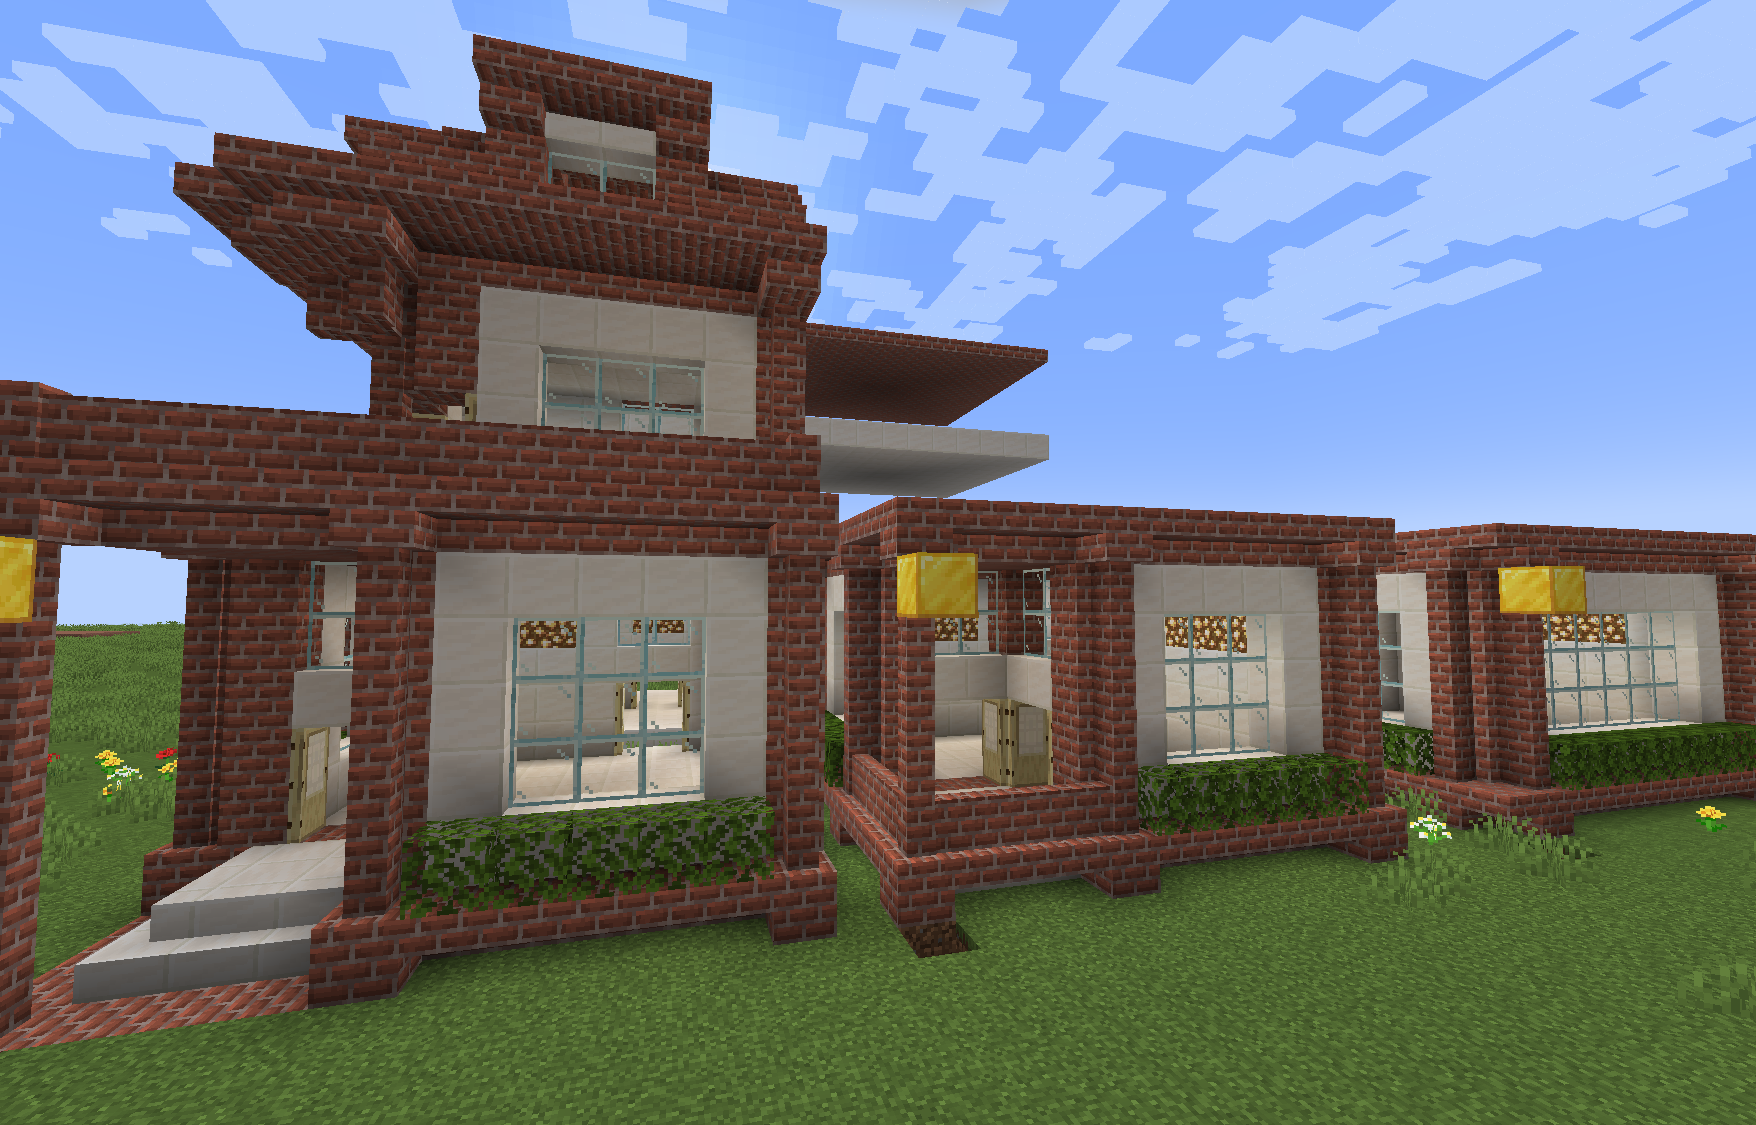
\includegraphics[width=\textwidth]{images/structures/building-strucutres-close-up.png}
    \caption{From left to right: building entrance corner, balcony and big window corner.}
    \label{fig_building_strucutres_close_up}
  \end{subfigure}
  \hfill
  \begin{subfigure}{0.48\textwidth}
      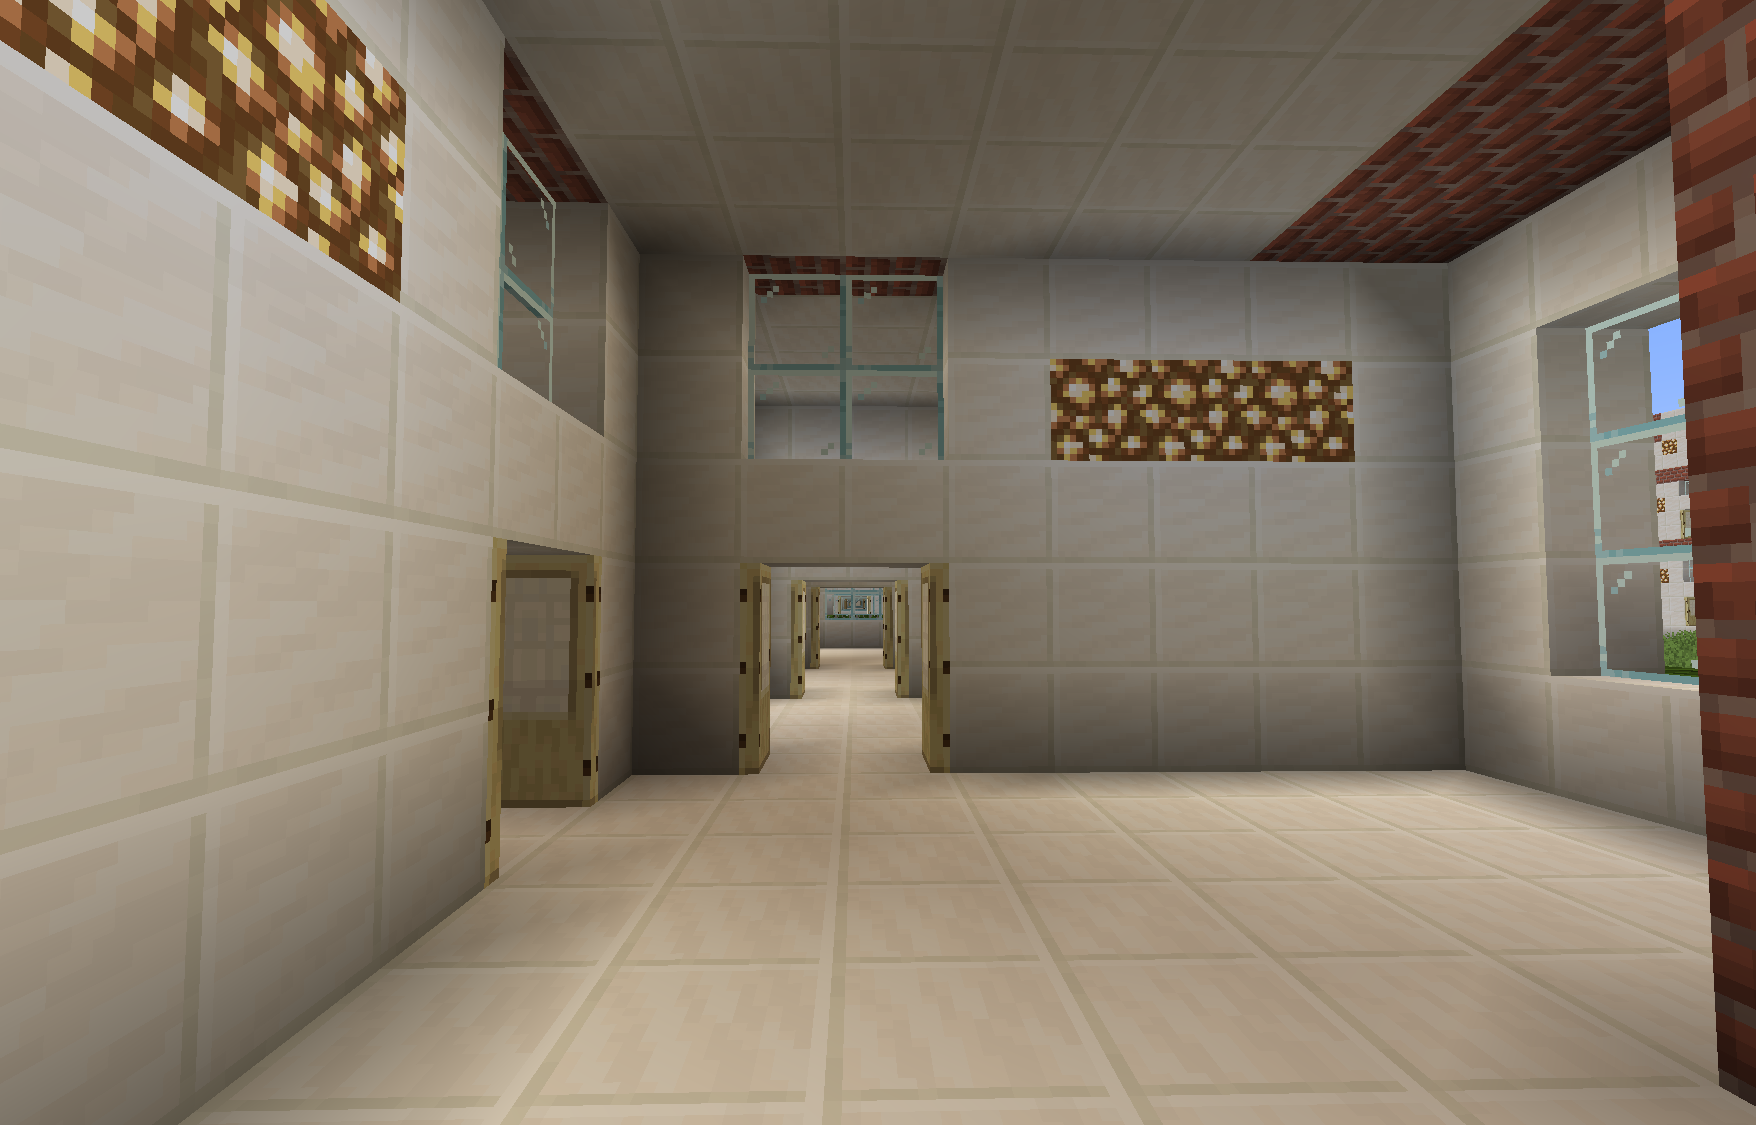
\includegraphics[width=\textwidth]{images/structures/building-strucutres-doors.png}
      \caption{Doors between each building structure.}
  \end{subfigure}
  \caption{Some manually designed building structures 
    which can be combined by placing them next to each other. 
    Doors between them are aligned to ensure accessibility of the whole building.}
  \label{fig_building_strucutres}
\end{figure}

% Structure scanning
In order to duplicate these structures, and apply translation and rotation onto them,
they need to be constructed using a computer program.
It was chosen to follow a scanner-builder approach over 
manually translating these structures into code that constructs them using 
simple geometry like cuboids 
because the scanner-builder approach is easier to implement 
and allows for faster iterations.
The scanner\footnote{\texttt{structure\_scanner.py}} works by 
serializing the user defined build area to a Python pickle file. 
Afterwards, the builder\footnote{\texttt{structure\_builder.py}} 
can be used to duplicate the scanned structure with arbitrary rotation and translation.
Every structure was scanned from the bottom left corner in positive XZ direction, 
by standing on the golden blocks shown in \autoref{fig_building_strucutres_close_up}.

% Structure building / placement (translations, roatations)
In total 14 building structures were designed, which are shown in figure \autoref{fig_building_strucutres_rotations}.
They are split between first floor ($11 \times 6 \times 11$) and roof house ($11 \times 9 \times 11$) elements.
There are simple corner elements and middle wall elements to allow building $n \times 2$
rectangular shaped buildings.
Additionally, center elements like \texttt{center} and \texttt{courtyard} were added to 
support $n \times m$ shapes. 
Later, the concept of an inner corner was added to allow for more complex shapes like  
$L$, $O$ and $+$.

\begin{figure}[ht]
  \centering
  \begin{subfigure}{0.48\textwidth}
    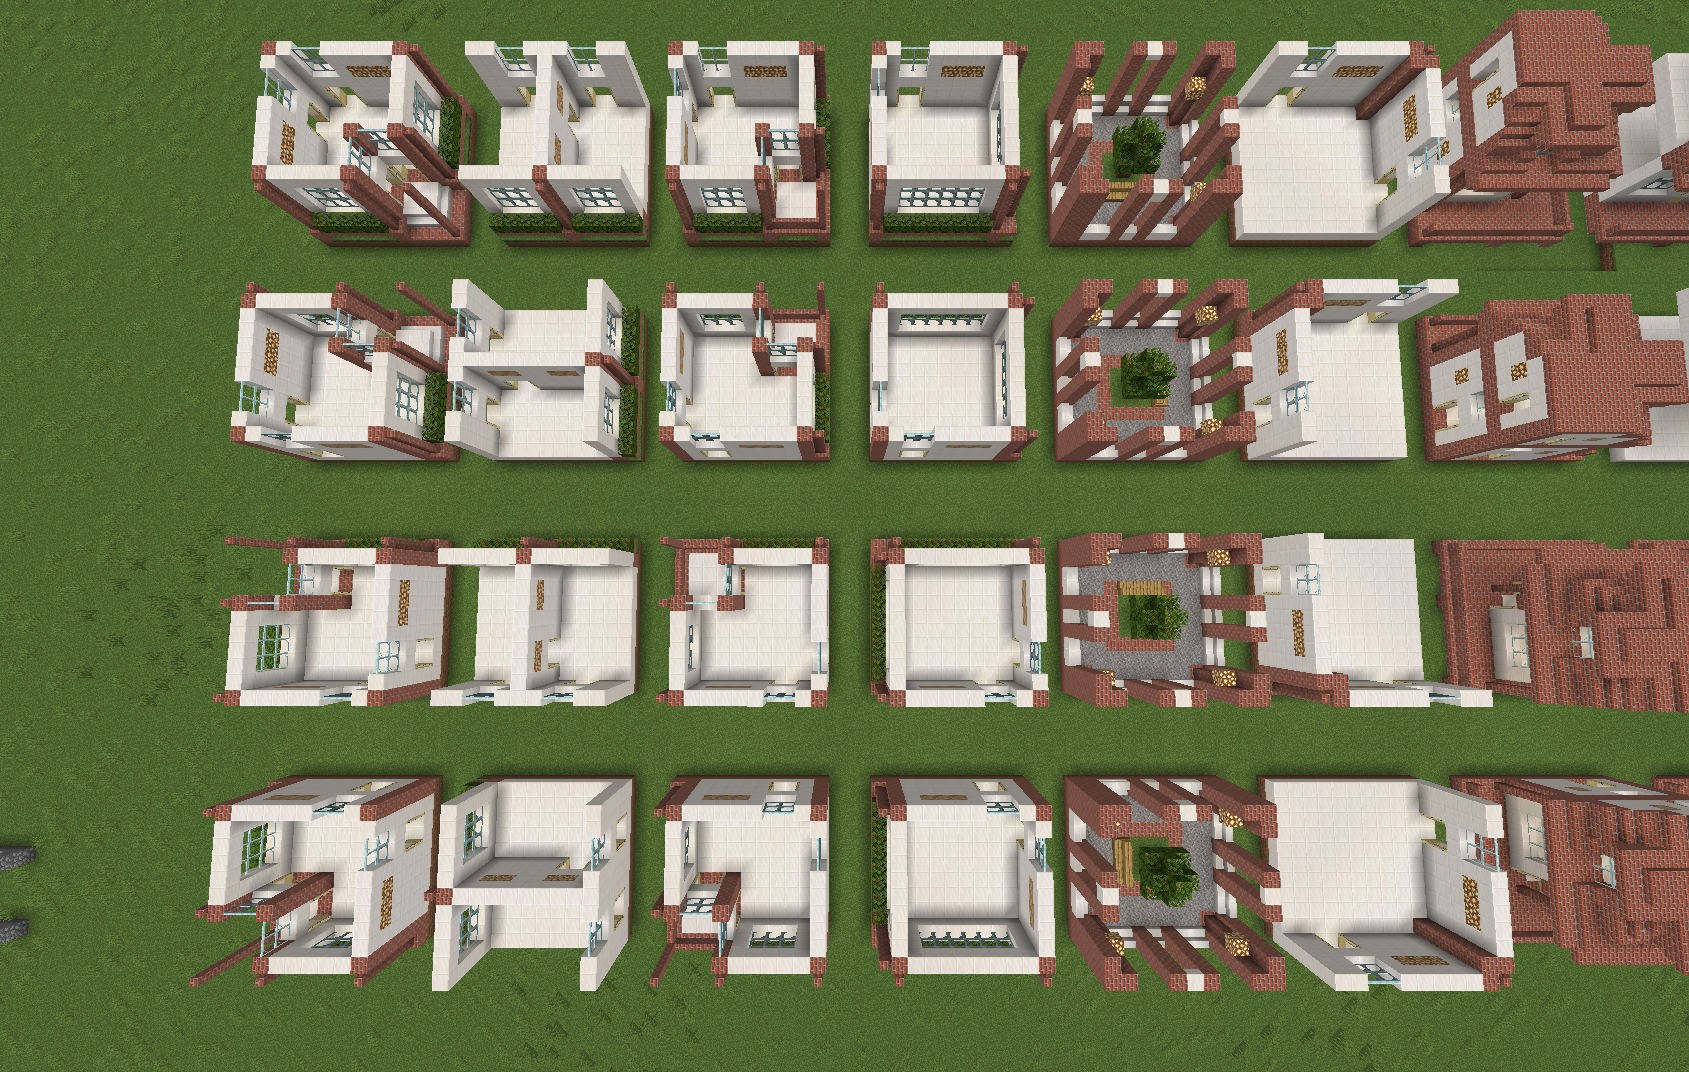
\includegraphics[width=\textwidth]{images/structures/buidling-strucutres-rotations-1.png}
    \caption{From left to right: building entrance corner, middle wall,
              balcony corner, big window corner, courtyard and inner corner.}
  \end{subfigure}
  \hfill
  \begin{subfigure}{0.48\textwidth}
      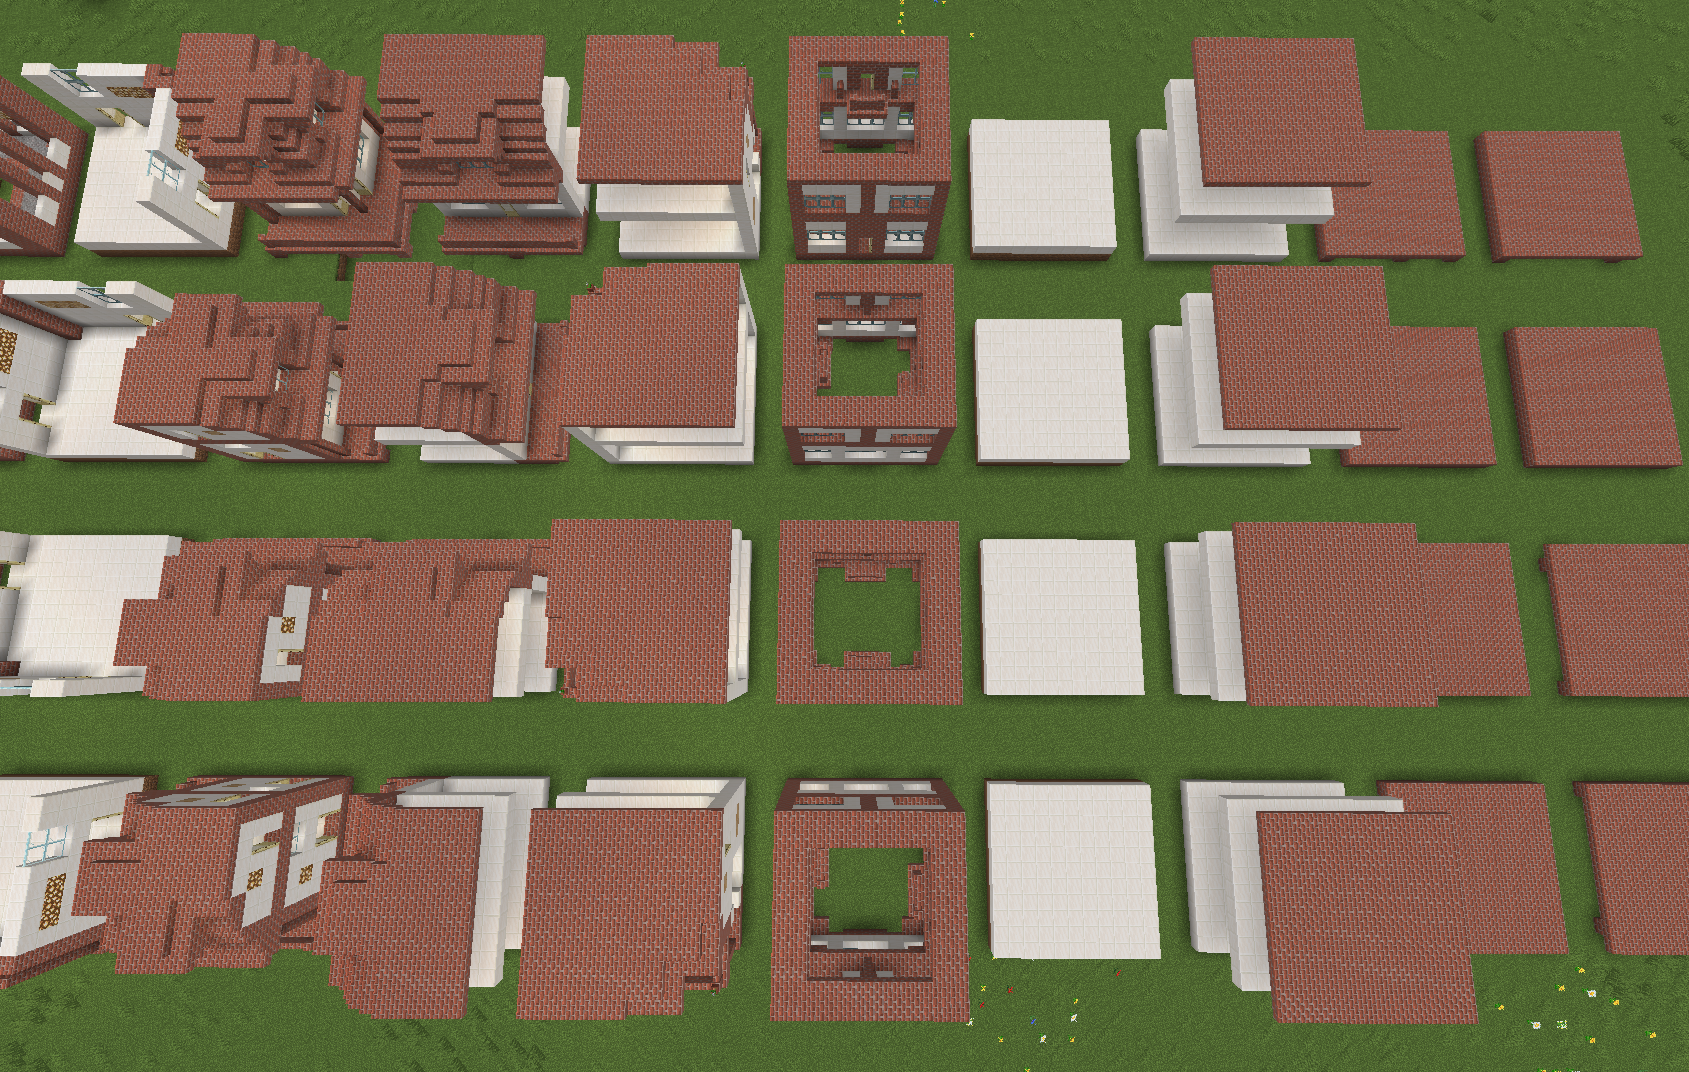
\includegraphics[width=\textwidth]{images/structures/buidling-strucutres-rotations-2.png}
      \caption{From left to right: corner roof house, middle wall roof house, inner corner roof house,
              courtyard roof house, center, center roof house, corner flat roof and big window flat roof.}
  \end{subfigure}
  \caption{All 14 designed building structures in all rotations. 
    Each column represents a single structure and 
    each of the four rows represent a rotation of that structure. }
  \label{fig_building_strucutres_rotations}
\end{figure}


With the introduced building structures one can already 
build whole houses by deterministically placing them next to each other, 
while making sure that all doors align as they are supposed to. 
Two examples are shown in \autoref{fig_deterministic_buildings}.

\begin{figure}[ht]
  \centering
  \begin{subfigure}{0.48\textwidth}
    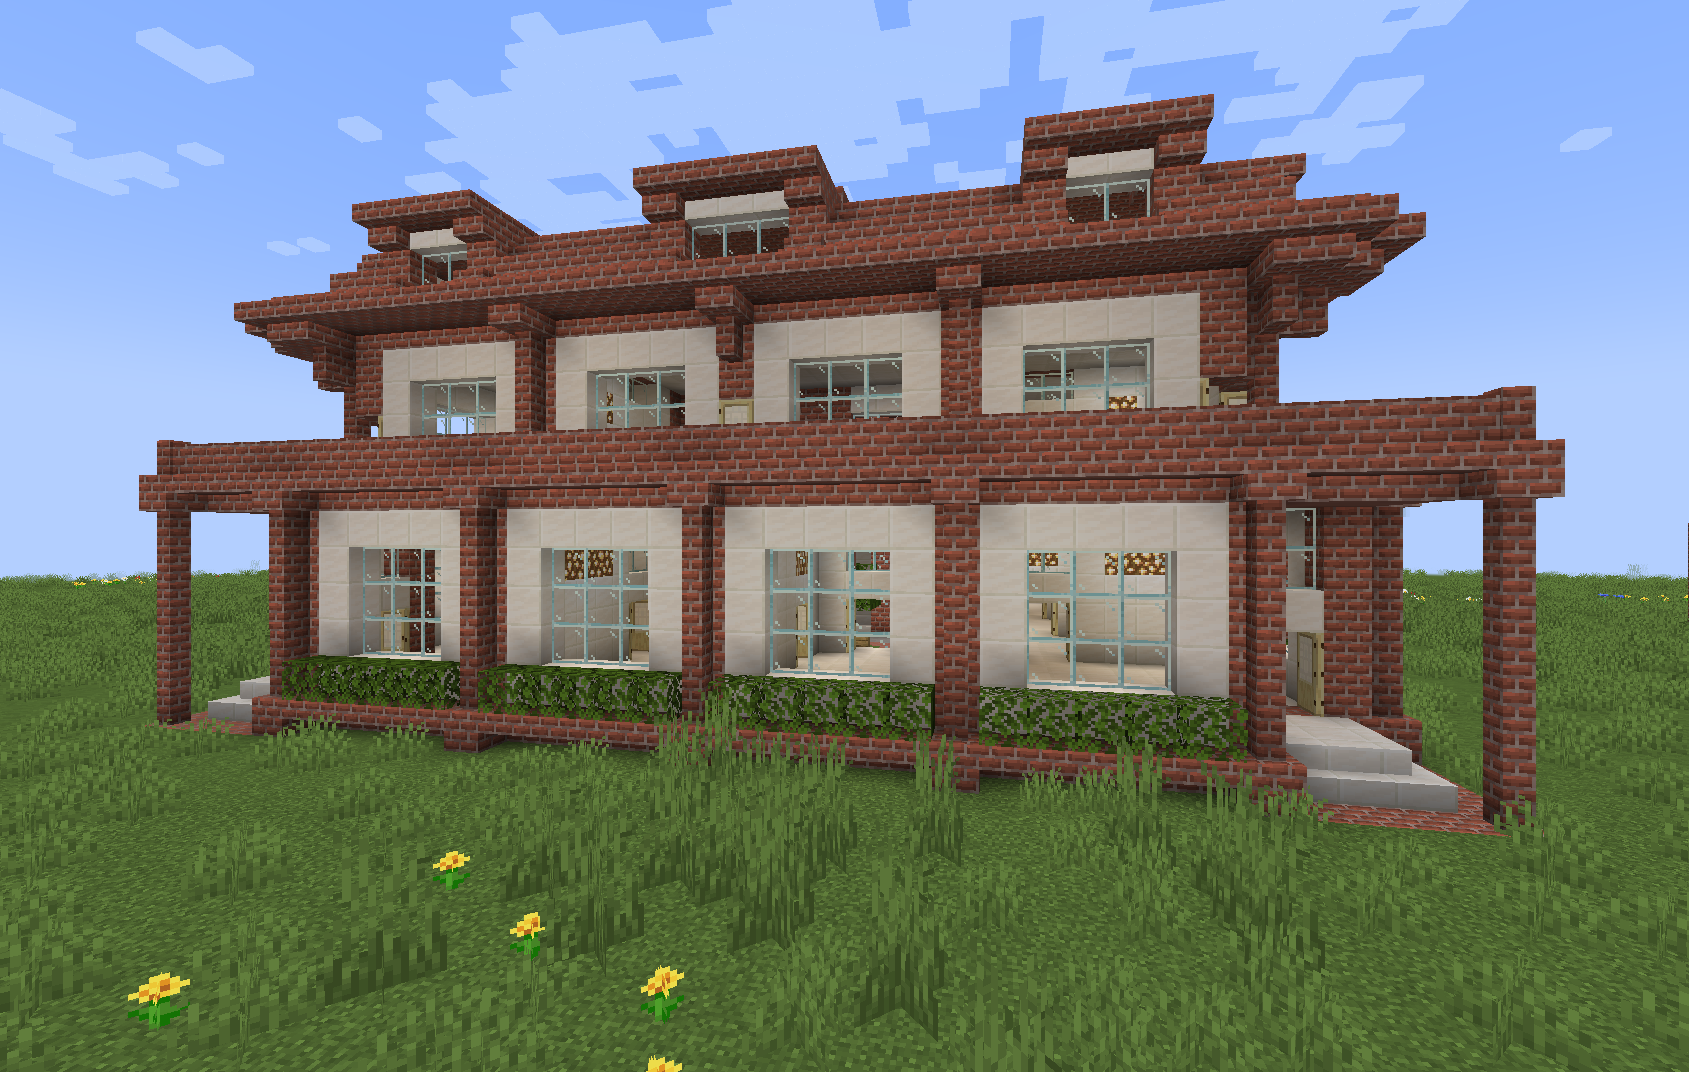
\includegraphics[width=\textwidth]{images/buildings/deterministic-building-with-roofhouse.png}
    \caption{A $3 \times 3$ house with courtyard and a second floor (roof house).}
  \end{subfigure}
  \hfill
  \begin{subfigure}{0.48\textwidth}
      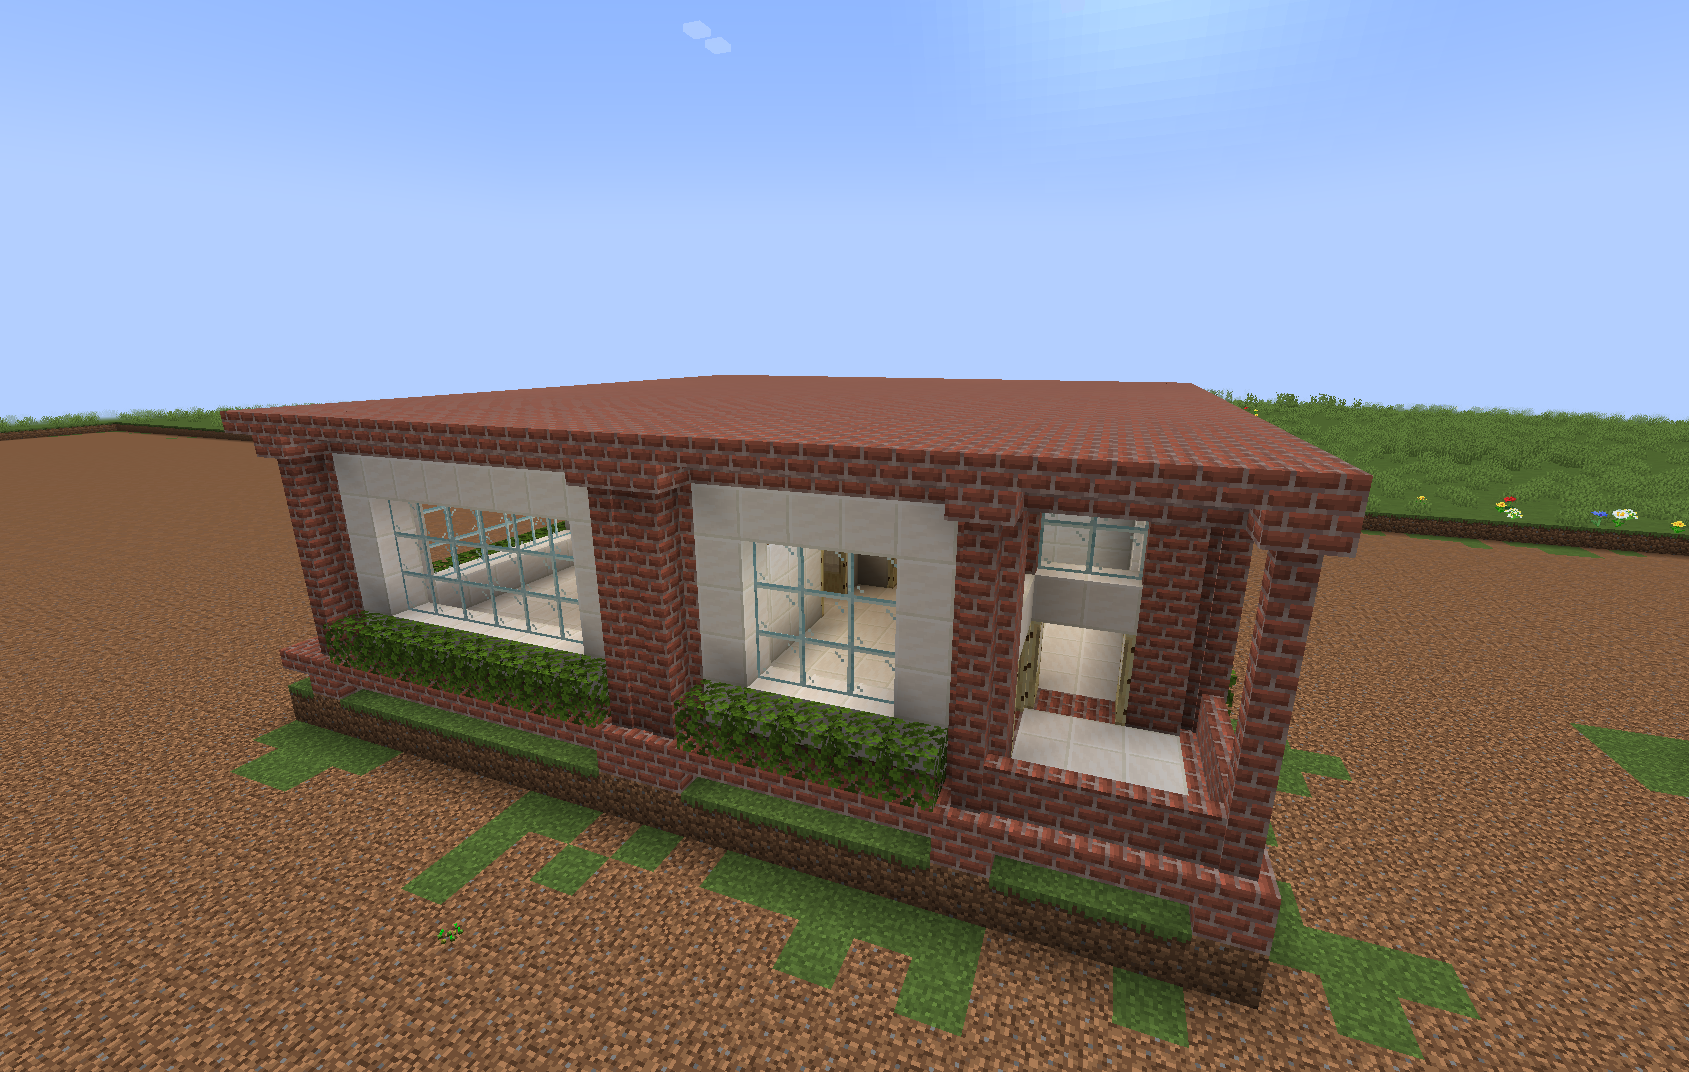
\includegraphics[width=\textwidth]{images/buildings/deterministic-building-with-flat-roof.png}
      \caption{A $2 \times 2$ house with a flat roof.}
  \end{subfigure}
  \caption{Two deterministically built buildings.}
  \label{fig_deterministic_buildings}
\end{figure}



\subsection{Wave function collapse}



% Symmetry checker

% Retry insteack of backtracking

% Air structures

% Air around building to enforce closed form

\section{Interior Design}

\section{Overall Results}

\section{Discussion}
% Summarize results
% Limitations
% Directions for improvement



%%%
%%% end main document
%%%
%%%%%%%%%%%%%%%%%%%%%%%%%%%%%%%%%%%%%%%%%%%%%%%%%%%%%%%%%%%%%%%%%%%%%%%%%%%%%%%%

\newpage
\appendix  %% include it, if something (bibliography, index, ...) follows below

%%%%%%%%%%%%%%%%%%%%%%%%%%%%%%%%%%%%%%%%%%%%%%%%%%%%%%%%%%%%%%%%%%%%%%%%%%%%%%%%
%%%
%%% bibliography
%%%
%%% available styles: abbrv, acm, alpha, apalike, ieeetr, plain, siam, unsrt
%%%
\bibliographystyle{alpha}

%%% name of the bibliography file without .bib
%%% e.g.: literature.bib -> \bibliography{literature}
\bibliography{literature}

\end{document}
%%% }}}
%%% END OF FILE
